\section{定位和层叠上下文}

\subsection{定位}
前面几章介绍了主流的三种文档流布局,定位不同于文档流,\texttt{position} 的默认值是 \texttt{static} 表示违背定位,如果设置了其他值,元素会被定位,也将彻底从文档流中移走。

\subsubsection*{固定定位}

固定定位最好理解,给一个元素设置\texttt{position: fixed}就能将元素放在屏幕视口的任意位置。这需要搭配四种属性一起使用:\texttt{top、right、bottom}和\texttt{left}。这些属性的值决定了固定定位的元素与浏览器视口边缘的距离。

固定定位的一个作用是使用脚本控制要填写的表单,但点击某个按钮时将 \texttt{display} 设置为非 \texttt{none} 值以显示表单。

\subsubsection*{绝对定位}

绝对定位 \texttt{display: absolute} 和固定定位的唯一区别是绝对定位是相对已定位的父元素块的,如果父元素未定位,则向上冒泡查找定位的元素。

\subsubsection*{相对定位}

相对定位 \texttt{display: relative} 不同于前两个定位值,它并没有让元素离开文本流,而是让元素相对于它本来的位置进行偏移。\texttt{top、right、bottom}和\texttt{left} 也不再指定元素与视口边距的位置,而是元素相对位移的位置。

\subsubsection*{粘性定位}

粘性定位,\texttt{position: sticky} 是相对定位和固定定位的结合: 正常情况下,元素会随着页面滚动,当到达屏幕的特定位置时,如果用户继续滚动,它就会“锁定”在这个位置。最常见的用例是侧边栏导航。


\subsection{层叠上下文}

浏览器将HTML解析为DOM的同时还创建了另一个树形结构,叫作渲染树(render tree)。它代表了每个元素的视觉样式和位置。同时还决定浏览器绘制元素的顺序。顺序很重要,因为如果元素刚好重叠,后绘制的元素就会出现在先绘制的元素前面。

浏览器会先绘制所有非定位的元素,然后绘制定位元素。默认情况下,所有的定位元素会出现在非定位元素前面。

\texttt{z-index} 属性的值可以是任意整数(正负都行)。拥有较高\texttt{z-index}的元素出现在拥有较低\texttt{z-index}的元素前面。拥有负数\texttt{z-index}的元素出现在静态元素后面。

给一个定位元素加上\texttt{z-index}可以创建层叠上下文。默认情况下,\texttt{z-index} 的值是 \texttt{auto},不创建层叠上下文。一个层叠上下文包含一个元素或者由浏览器一起绘制的一组元素。其中一个元素会作为层叠上下文的根,比如给一个定位元素加上\texttt{z-index}的时候,它就变成了一个新的层叠上下文的根。所有后代元素就是这个层叠上下文的一部分。

使用层叠上下文有一个注意点,如果有两个父元素\texttt{one} 和 \texttt{two},他们的 \texttt{z-index} 值为 \texttt{1}, 后定义的元素(\texttt{two})会出现在先定义的元素上方(顺序覆盖)。如果 \texttt{one} 中有一个元素 \texttt{element} 的 \texttt{z-index} 值为 100,他也可能显示在 \texttt{two} 的下方,子元素的 \texttt{z-index} 值只再父元素内产生层叠优先级影响,对父元素本身没有影响。

\begin{figure}[H]
    \small
    \centering
    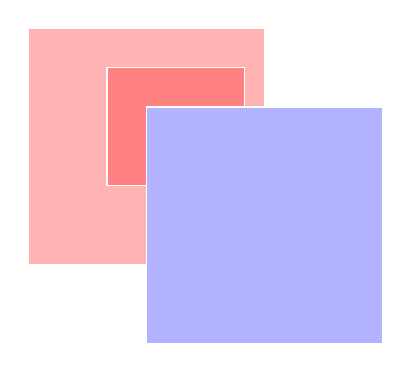
\begin{tikzpicture}[scale = 1]
        \draw[color = white, fill = red!30] (0,0) rectangle (3,3);
        \draw[color = white, fill = red!50] (1,1) rectangle (2.75,2.5);
        \draw[color = white, fill = blue!30] (1.5,-1) rectangle (4.5,2);
    \end{tikzpicture}
    \caption{\texttt{z-index}}
\end{figure}

所有层叠上下文内的元素按照如下顺序叠放:
\begin{itemize}
    \item 层叠上下文的根
    \item \texttt{z-index} 为负的定位元素(及子元素)
    \item 非定位元素
    \item \texttt{z-index} 为\texttt{auto}的定位元素(及子元素)
    \item \texttt{z-index} 为正的定位元素(及子元素)
\end{itemize}

在实际开发中,一般不会直接给 \texttt{z-index} 设置一个具体的数值,如果 \texttt{z-index} 被使用多次,这会让代码很难维护,根本不知道元素,根元素的层叠顺序。更推荐统一管理 \texttt{z-index},比如这种做法:

\begin{HTML}
:root {
    --z-loading-indicator:  100;
    --z-nav  -menu:         200;
    --z-dropdown-menu:      300;
}

nav {
    z-index: var(--z-nav);
}
\end{HTML}

\newpage